\begin{frame}{Introduction}\section{Introduction}
	\begin{columns} \hfill
		\begin{column}{0.5\linewidth} \centering
			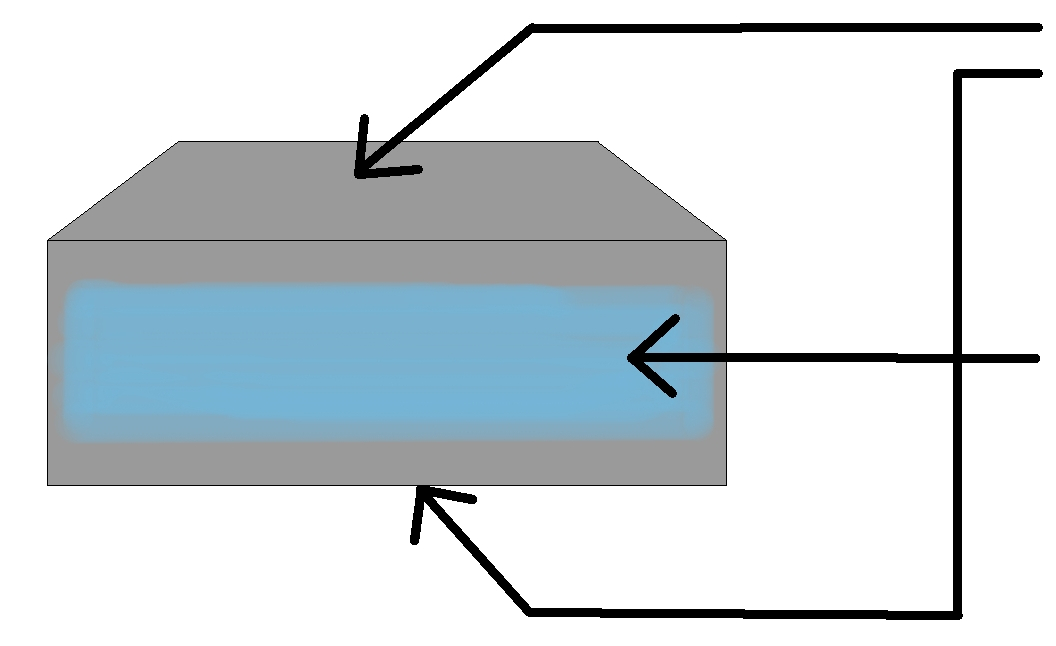
\includegraphics[width=.7\linewidth]{extrabilder_fuer_vortrag/Introduction1.jpg}
		\end{column}
		\begin{column}{0.5\linewidth} 
			conducting surface states
			
			\vspace{23px}
			insulating in the bulk
			
			\vspace{28pt}
		\end{column}\hfill
	\end{columns}
	\note{HgTe \\}
	
	\begin{columns}
		\begin{column}{0.1\linewidth}
			\vspace{9px}
			$0.5 \unit{nm}~\approx$
		\end{column}
		\begin{column}{0.8\linewidth}
			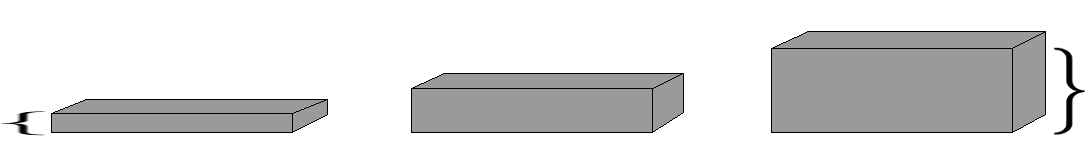
\includegraphics[width=\linewidth]{extrabilder_fuer_vortrag/Introduction2.jpg}
		\end{column}
			\hspace{-15px} 
		\begin{column}{0.1\linewidth}
			\vspace{.2px}
			$\approx~2.7 \unit{nm}$
		\end{column}
	\end{columns}
	\note{Hier steht, was ich zu bild 2 sage}

\end{frame}

%%% Local Variables:4
%%% mode: latex
%%% TeX-master: "main_BA2_Vortrag.tex"
%%% End: